\documentclass[11pt, a4paper]{article}
\usepackage{lmodern}
\usepackage[utf8]{inputenc}
% \usepackage{fontspec}
\usepackage{amssymb,amsmath}
\usepackage[T1]{fontenc}
\usepackage[scale=0.7]{geometry} 
\usepackage[french]{babel}% pour un document en français.
\usepackage{minted}
\usepackage{graphicx}
\usepackage[colorlinks=true, linkcolor=blue]{hyperref}
\date{}
\title{Rapport de TP de Technologie Web Serveur}
\author{Loïc \textsc{Castillo} Loris \textsc{Croce}}

\begin{document}

\maketitle

\section{Conception}

\begin{figure}[!h]
   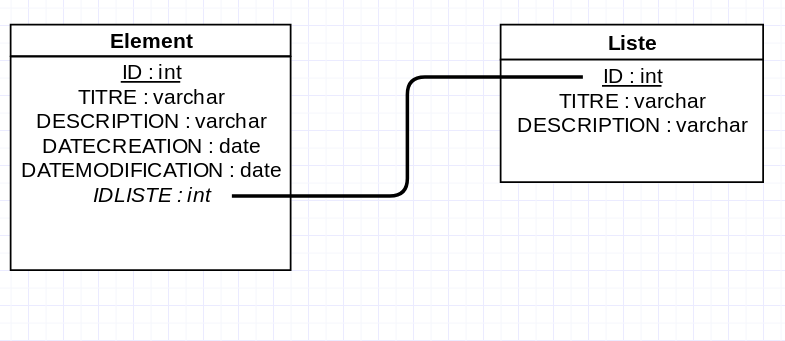
\includegraphics[width=15cm]{donnees.png}
   \caption{Modèle de données}
\end{figure}

\paragraph{Ressources} On interagira avec des listes et des éléments qui pourront être affichés (un élément affiché dans une liste), ajoutés, supprimés et modifiés.

\paragraph{Espaces de noms} Pour l'affichage seules les listes auront une URL de la forme : \texttt{/liste/\emph{nomDeLaListe}}




\section{Modèle et accès au données}

Nous avons donc deux classes métiers pour le modèle : \verb|Element| et \verb|Liste| définissant les deux objets manipulés.\\ 

Étant donné que le nombre d'appels à la base de données ne sera pas très élevé, nous avons décidé que notre DAO serait une classe statique. Les informations pour se connecter à la base de données sont stockées dans les variables de la classe. Chaque fonction retourne des objets métiers et est utilisée pour une tâche précise (ex: récupérer toutes les listes, les éléments, un élément particulier, les éléments en fonction de leur liste\dots). Chaque appel de fonction doit recréer une connexion à la base de données.

\section{Représentations}

Via FreeMarker, nous avons créé 3 templates :
\begin{itemize}
	\item \verb|complet.ftl|, qui affiche tous les éléments de toutes les listes.
	\item \verb|listeDetail.ftl|, qui affiche une liste donnée et tous ses éléments. Elle permet de supprimer ou de modifier des éléments.
	\item \verb|listes.ftl|, qui fait office de page ``d'accueil'' en affichat un tableau des listes. Elle permet également de d'ajouter, modifier ou supprimer des listes, ajouter des éléments.
\end{itemize}

\section{Interactions}

Pour la gestion des interactions par le contrôleur avec Spark nous n'avons utilisé que deux méthodes HTTP : GET et POST. En effet, la gestion de méthodes telles que DELETE ou PATCH ne s'est pas révelée assez pertinente en raison de leur plus complexe mise en place. On a donc un ensemble de \emph{routes} de types \verb|get| pour récupérer du contenu ou supprimer des élements (on affiche la liste en enlevant l'élement voulu). Ainsi qu'un ensemble de \emph{routes} \verb|post| pour créer ou modifier du contenu.

\section{Ajout de fonctionnalités}

\paragraph{Statut optionnel} Il suffit d'ajouter une table \verb|Etat| dans la base de données, contenant un id et un varchar, qui contiendrait 3 tuples, dont la valeur des varchar serait : soit \emph{à faire}, \emph{fait} ou \emph{supprimé}.

\paragraph{Sous-listes}
Dans la BDD, la table \verb|Liste|, aurait une colonne \verb|Upper|, qui contiendrait l'ID d'une autre liste, ou serait NULL.
En Java, cela se matérialiserait par l'ajout d'une List de Liste dans la classe Liste. Celle-ci serait vide si l'attribut est NULL dans la BDD.

\paragraph{Élément appartenant à plusieurs listes}
Dans la BDD, il faudrait créer une table de liaison, qui lirait deux listes. On pourrait l'appeler \verb|ListJunction|, et serait composer de deux id de Liste. L'ajout de ces deux id donneraient la clé primaire de l'élément.

\paragraph{Étiquette} En Java : \verb|List<String>| dans chaque élément correspond aux tags.
En BDD : Ajout d'une table \verb|Tag [ id : long (PRIMARY KEY), text : varchar]|.
Ajout d'une table pour unir un Tag à un Element. Cette table contiendrait en attribut l'id d'un tag et d'un element, et sa clé primaire serait la concaténation des deux.


\end{document}